\chapter{Work}
\label{chap:work}
% **************************** Define Graphics Path **************************
\ifpdf
    \graphicspath{{Chapter3/Figs/Raster/}{Chapter3/Figs/PDF/}{Chapter3/Figs/}}
\else
    \graphicspath{{Chapter3/Figs/Vector/}{Chapter3/Figs/}}
\fi

The aim of this study was to capture the iterative elongation process
of even-chain saturated Fatty Acids. Fatty Acids are
carboxylic acids with long hydrocarbon side groups
(Figure~\ref{fig:fas}) and they are usually characterised by the
number of carbons in these side-groups, for example a FA with a chain
of 6 carbons is usually denoted as $C_6$. The side-chains of FAs grow
by successive $C_2$ concatenations. This concatenation process takes places at
the FA biosynthesis pathway in the cytosol for chain lengths up to
$C_{18}$. Further elongation takes places at the FA elongation
pathway in the Endoplasmatic Reticulum(ER).

\begin{figure}[htbp!]
\centering
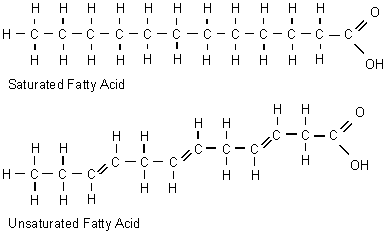
\includegraphics[width=0.6\textwidth]{fas}
\caption[Fatty Acid structure]{The structure of Fatty Acids(FA) which
  consists of a long hydrocarbon side-group. The length of this
  side-group charactersises the FA.}
\label{fig:fas}
\end{figure}

In this study we are interested in the elongation process in its
entirety so our models capture the combined effect of the two pathways
responsible for it, FA biosynthesis \textit{and} FA elongation. In
this section I first introduce the basic model and the assumptions
made to simplify it, the tuning of that basic model based on FA
measurements, a version of the model in stochastic pi-calculus and
finally the extension of the model with the introduction of some
control mechanisms.

\section{Basic model}
\subsection{Petri Net implementation}
\label{sec:pn_implementation}
FA biosynthesis starts with Acetyl-CoA which is being converted to
Malonyl-CoA. A reaction between Malonyl-CoA and Acetyl-CoA starts off
the first $C_4$ FA product and a $CO_2$ molecule. After that there are successive $C_2$
concatenations to elongate the FA product with each elongation step
that requires 4 reactions, requiring another Malonyl-CoA(Figure~\ref{fig:fa_synthesis}). The
full pathway from KEGG can be seen in
Figure~\ref{fig:kegg_synthesis}. The elongation pathway located in ER
is similar in nature but the intermediaries are CoAs instead of
ACPs (Figure \ref{fig:kegg_elongation}). ACPs (Acyl Carrier Proteins)
is where the growing FA chain is bound during elongation. 

\begin{figure}[htbp!]
\centering
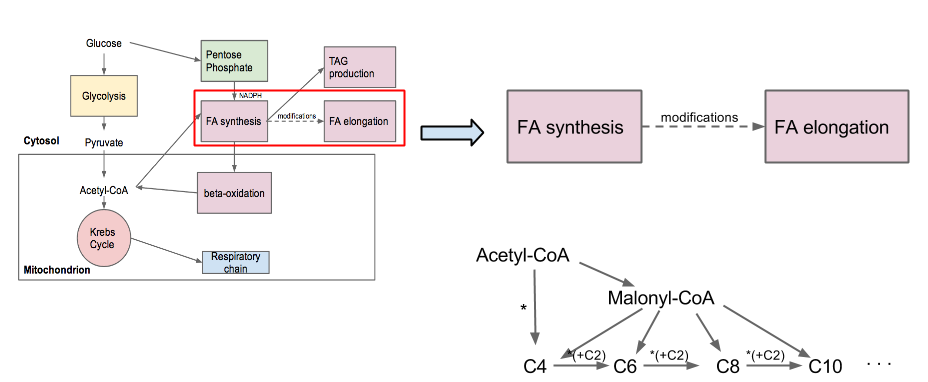
\includegraphics[width=1.0\textwidth]{fa_metabolism}
\caption[FA metabolism]{FA metabolism in relation to other pathways.}
\label{fig:fa_synthesis}
\end{figure}

\begin{figure}[htbp!]
\centering
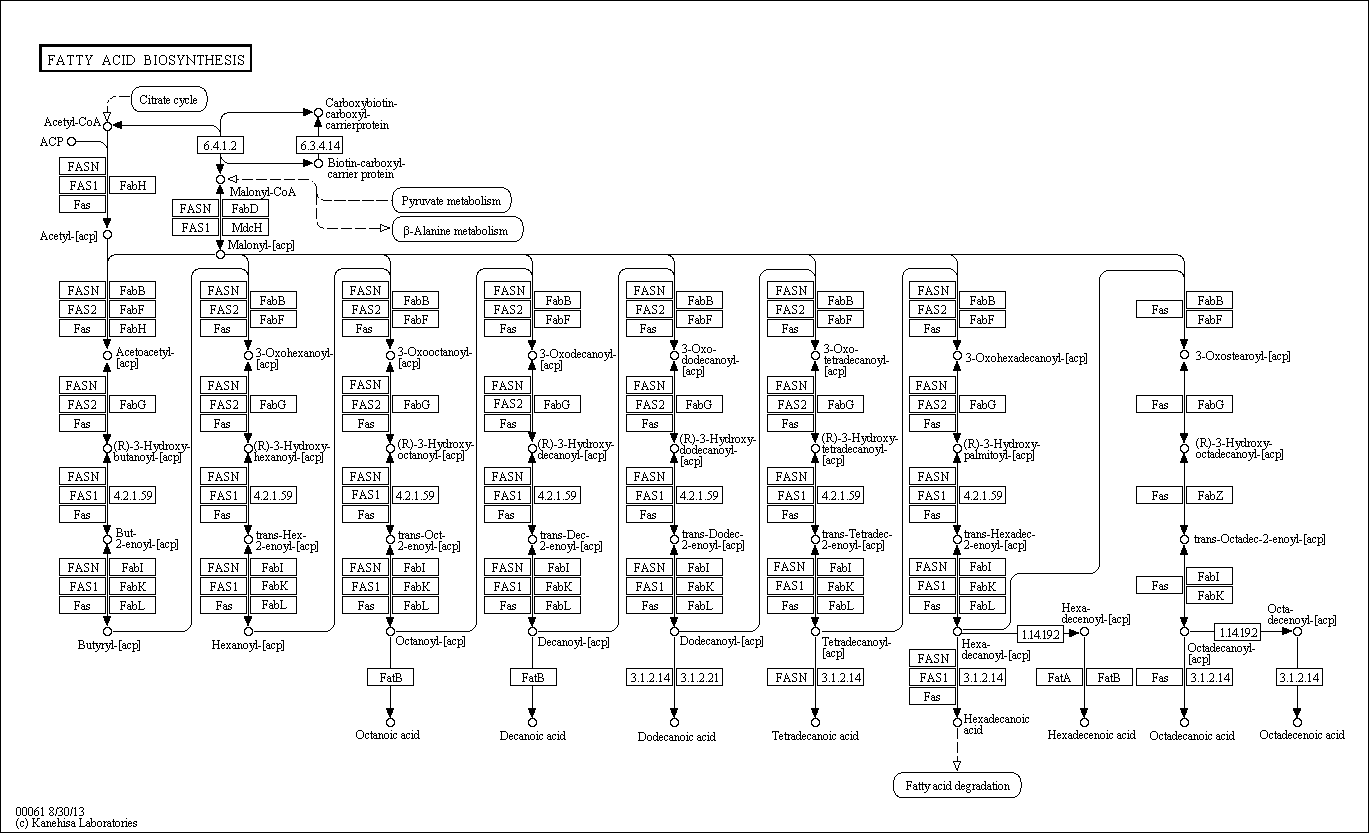
\includegraphics[width=1.0\textwidth]{kegg_synthesis}
\caption[Fatty Acid biosynthsis in cytosol]{FA biosynthesis in the
  cytosol. Notice the successive concatenations. Each concatenation
  takes 4 reactions.}
\label{fig:kegg_synthesis}
\end{figure}

\begin{figure}[htbp!]
\centering
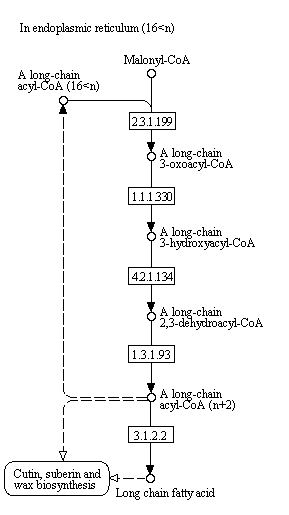
\includegraphics[width=0.3\textwidth]{kegg_elongation}
\caption[Fatty Acid elongation in ER]{General form of FA elongation in
ER. Notice that the intermediate products are CoAs instead of ACPs as
in biosynthesis.}
\label{fig:kegg_elongation}
\end{figure}

Because of the natural correspondence between biochemical reactions as
they are annotated in the KEGG static model to Petri Net model constructs
a straight translation between the two is straightforward. All the
pathway reactions become transitions with pre-places the reactants and
post-places for the products. Here we made our first assumptions by
omitting the enzymes participating as catalysts from the reactions. Information about the enzymes
is not so important for our purposes since we are interested in the
numbers of molecules of the metabolites involved in the process. Information
about the enzymes can be incorporated in the transition rates.
The net can be animated using its formal
operational semantics and as transitions/reactions occur
tokens/metabolites move through the net. The FA products are
represented as sinks, places that are not pre-places to any
transition, so once a token reaches one of these sinks it is
trapped. That way the probabilistic iterative nature of the process is
captured completely, an intermediate of the process can either remain
at that length or go on to form longer FAs. The sinks are therefore
the outputs of the stochastic process with the inputs being the places
that do not act as post-places for any transition. Starting with some
finite number of molecules at the inputs, these will be consumed
throughout the process until we reach a dead-state where no further
transitions are enabled. The translation from the KEGG pathway model
to the Petri Net model was done manually with the SNOOPY \cite []
{heiner2012snoopy}tool which
allows you to draw a net, play the token game for basic nets to
observe its behaviour, and get the dynamic behaviour of the
metabolites over the integration time.

\begin{figure}[htbp!]
\centering
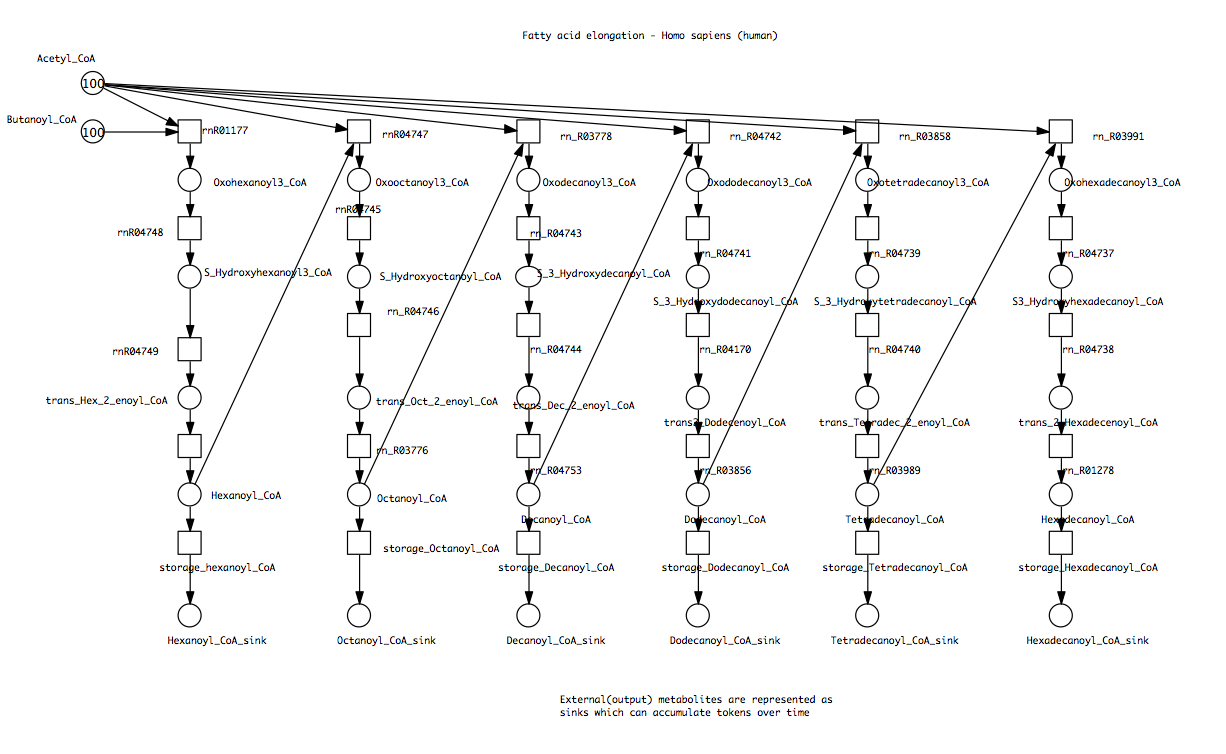
\includegraphics[width=1.0\textwidth]{pn_fa_elongation}
\caption[FA elongation Petri Net model]{}
\label{fig:pn_fa_elongation}
\end{figure}

A direct translation from KEGG is certainly useful for capturing a
low-level biochemical view of the system. The model can offer an even
more fine-control view of the system than the model presented in
Figure~\ref{fig:pn_fa_elongation} by including the enzymes in the
reactions and information about their activity to the reaction
substrates. However including too many details in the model can
sometimes hide the true aspect of the system the modeller is trying to
understand and analyse. Here we are interested in the probabilistic,
non-deterministic nature of the iterative FA elongation process which
happens as this series of $C_2$ concatenation steps in FA elongation
and biosynthesis pathways in ER and cytosol respectively. The outputs
we are particularly interested to see are the numbers and proportions of FAs at
different lengths. In Petri Nets model language these are the number
and more importantly the proportions
of molecules/tokens that end up in the sink places at the stop of the model
execution. Because the process is inherently iterative and
probabilistic these numbers will be different at the end of each model
execution and in the limit the average number of metabolites will be
the same as the equivalent deterministic model. This is in contrast with most dynamic modelling approaches
as we are not interested in the time traces but rather only at the end
result of this stochastic process and matching with the experimental
dat awe have afterwards. We can think of the Petri Net as a
magic box governed by some probabilities(that we can tune) where we
throw some inputs and according to these probabilities some output
will come out at the other end in the form of proportions of FAs at different
lengths. The probabilities are just the control parameters that guide
the operation of the magic box.

Having outlined our modelling goals in the previous section we can now
make some assumptions that will guide our design of the simplified
synthesis/elongation model that will be our basic model throughout
this study. First of all the model will capture the combined effect of
both pathways. The two pathways are in different compartments of
the cell, one in cytosol and one in ER, but we will ignore the
transportation of FAs from cytosol to ER and we will assume that the
two process are sequential so a $C_{18}$ for example can be elongated
directly to a $C_{20}$ while in reality it would have to first be
transported to the ER. Since we also take this view of the
net model as a control box turning input signal through a series of
steps to an output signal, we can safely squeeze the four step reaction chain
needed for each $C_2$ concatenation step to a single step reaction and
at the same time consider only the forward direction
reactions. Also, since we no longer consider exact chemical
reactions we will consider constant values for the the reactions rate
functions and we will treat those as probabilities that will govern the
non-deterministic decisions during the execution of the model. Finally we
also decided to stop the elongation process at $C_{22}$. Therefore the
sinks will only include products $C_{12}$ - $C_{22}$. FAs with lengths
4-10 will be included but no output will be considered. These
decisions are supported by the output from the real experimental data available
for tuning the model (see
Results section).

The basic model was built with SNOOPY \cite [] {heiner2012snoopy} using the previous conditions and assumptions. This basic model that will
be the basis for our work in this study can be seen in
Figure~\ref{fig:fa_elongation_full}. The model is similar in nature to
the more full model presented previously but the concatenation steps
are represented as single transitions and the elongation process goes
up to $C_{22}$ because the elongation process in the ER is also
included. Initially, I consider as simple model with two input points Malonyl-CoA
and Acetyl-CoA whereas in reality the only precursor of FA
biosynthesis is Acetyl-CoA and the 2 input points of the pathway are
products coming from Acetyl-CoA. The model as presented in
Figure~\ref{fig:fa_elongation_full} starts with inputs: 300
Malonyl-CoA and 100 Acetyl-CoA molecules. The model can then be set in
motion with SNOOPY until it reaches a dead state which 
corresponds to the point where the system runs out of input
metabolites to 'fuel' further reactions. The output of the system
is the number of tokens accumulated at each sink or FA of
different lengths.

\begin{figure}[htbp!]
\centering
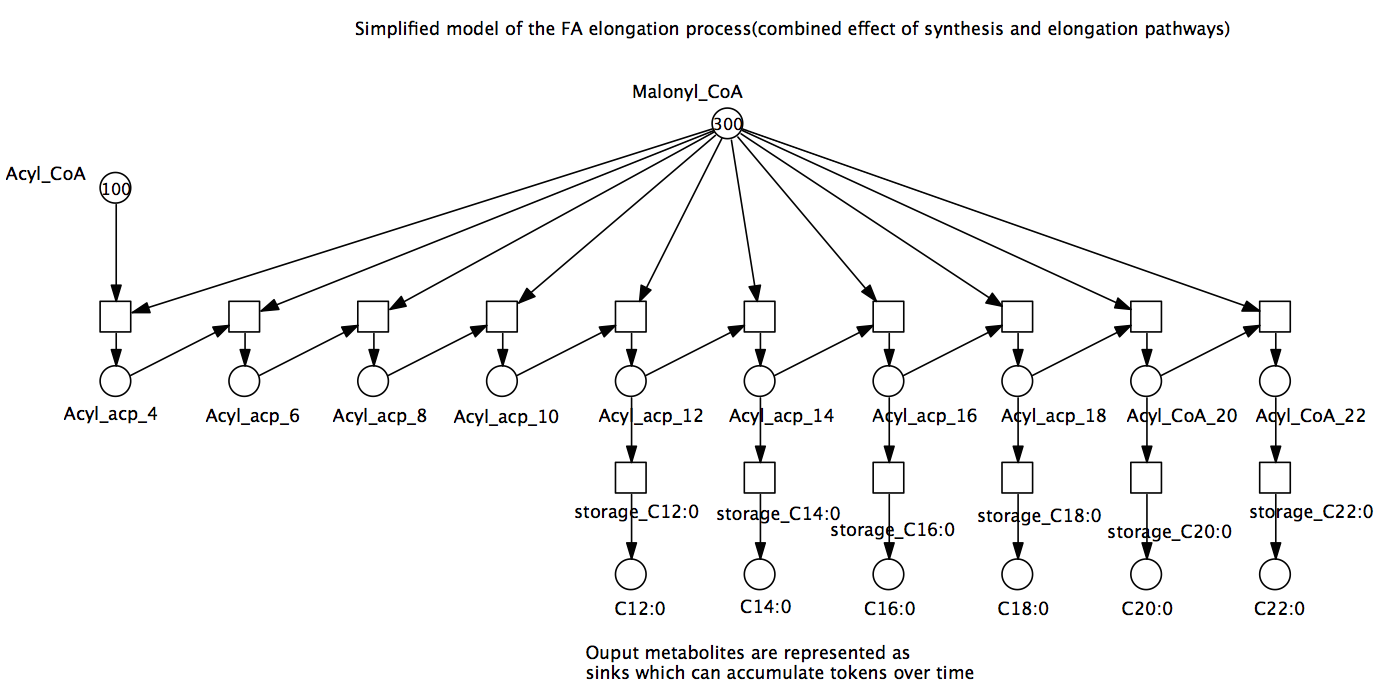
\includegraphics[width=1.0\textwidth]{fa_elongation_full}
\caption[Petri Net implementation(basic model)]{Petri Net
  implementation of the basic model as described in the main text}
\label{fig:fa_elongation_full}
\end{figure}


Observing the execution pattern of the basic net model we notice an
execution pattern which leads to an elegant view of the system as a
series of binary probabilistic decisions or Bernoulli trials. At the start of the model
execution only the initial transition producing the first product $C_4$ is
enabled. If we consider that after this transition it
will only fire again after its initial product has reached a sink then
at each iteration only one token is travelling through the net. This token
goes through an iteration of repeating the same binary decision: to either stay at the current length or continue to form a longer FA. More formally as the token gets
transformed to an intermediate product there are only two transitions
enabled: the transition taking it to the next longer intermediate and
the transition taking to be stored at its current length(Figure~\ref{fig:binary_decision}). Let these
two transitions be $t_1$ and $t_2$ respectively. According to
the operational semantics of Stochatic Petri Nets (see Section~\ref{sec:spn})
a wait time is sampled for each of the enabled transitions from a
negative exponential distribution with rate the value of the rate
function of the
transition. In this case the rate function of the two transitions are
constants (see assumptions) $\lambda_{t_1}$ and $\lambda_{t_2}$. Since
we know that one of the reactions will fire we can say that the
firing probabilities of the two transitions or the probabilities of
the token's decisions are:

\begin{align*}
P(staying)& =P(t_1) = \frac{\lambda_{t_1}}{\lambda_{t_1} + \lambda_{t_2}}\\
P(continuing) & = P(t_2) = \frac{\lambda_{t_2}}{\lambda_{t_1} + \lambda_{t_2}} = 1 - P(t_1)\\
\end{align*}


\begin{figure}[htbp!]
\centering
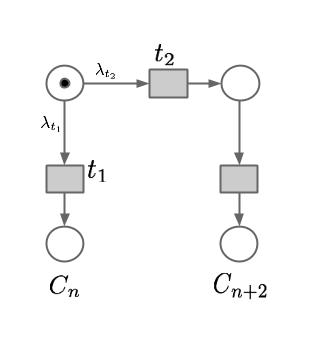
\includegraphics[width=0.5\textwidth]{binary_decision}
\caption[Binary stay-continue decision]{Binary decision at a
  particular point in the execution.}
\label{fig:binary_decision}
\end{figure}

In other words this is a Bernoulli trial with probability of success
$p = P(t_1)$. Since we only considered the outputs at the end of the
execution and not the timeframe of the process from start to finish,
then only the ratio of these two successive transitions rates is
important and not their absolute numbers. The entire journey of a token through the network
from the initial $C_4$ product until it reaches a sink and gets stored,
can be thought of a series of Bernoulli
trials(Figure~\ref{fig:trials}). The entire stochastic process
can be thought of a sequence of successive realisations of this series
of trials with tokens travelling through the net one
after the other with each one going through the series of decisions
or Bernoulli trials. The initial assumption that only one token
travels through the net at each time can in fact be dropped since the
output of the net only depends on the ratios of the pair of
transitions representing each binary decision. We consider this assumption, because it is intuitive and reduces the  problem to a successive realisations
of chains of Bernoulli trials.
It is also interesting to note how the binary decision
corresponds to a conflict between two events that share pre-conditions
which create non-determinsim through a race condition between the two
depdendent events. The 'conflict' that represents this decision
process is captured inherently in the structure and semantics of Petri
Nets.

\begin{figure}[htbp!]
\centering
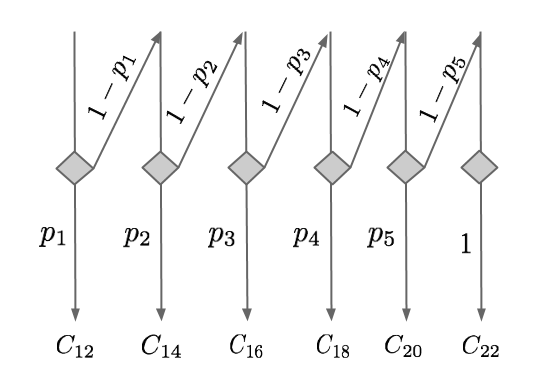
\includegraphics[width=0.55\textwidth]{trials}
\caption[Stochastic proces as a series of Bernoulli trials]{The entire
stochastic process a series of Bernoulli trials.}
\label{fig:trials}
\end{figure}

Each realisation of the stochastic process described by the Petri Net
model is itself a series of successive realisations of series of
Bernoulli trials that have different outputs. While SNOOPY is a great
tool for the visual side of the process, creating the model and animating
it, in order to be able to execute the model many times and with many
orders of multiple iterations to get
output profiles we needed a programmatic solution. We wrote code in
Python that can read a model, execute it once or a number of times, and write
out the results. For the description of the model I used the PySCeS
model description language for biochemical systems which is aimed at
the Python language \cite [] {olivier2005modelling}. The reactions are
defined in the standard chemical notation and since this corresponds
exactly to Petri Net transitions it was easy to load the description
into an appropriate Petri Net representation (Figure~\ref{fig:code}).

\begin{figure}[htbp!]
\centering
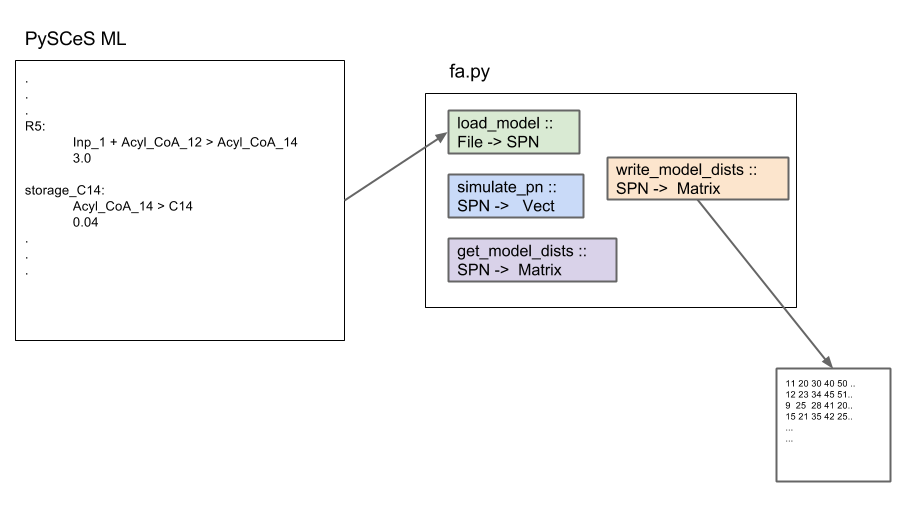
\includegraphics[width=1.0\textwidth]{code}
\caption[Workflow]{Structure of the code and workflow.}
\label{fig:code}
\end{figure}


\subsection{Model parameters}
\label{sec:params}
In Section~\ref{sec:pn_implementation} we described the building of the basic model
based on the goals and assumptions of the study. The elongation aspect
that we are interested in was reduced down to a sequence of successive
series of Bernoulli trials to determine the length that a FA will
stop its elongation at. The interesting parameters of the model, the
ones that will affect the output, are the success probabilities for
the stay-continue decisions for FA intermediaries with lengths
$[C_{12}, C_{22}]$ since they are ones that have sinks. In this
section two methods are presented for the identification of these parameters for
tuning the model so that its execution is biologically valid. They both rely on having experimental real dataset of
realative proportions of FAs. These data can be
seen as different realisations of the stochastic process that acts in nature. The attempt is then to tune our
model to be as close to the real model as possible by trying to tune
the proportions of the outputs of our model to match the proportions
of the outputs by the in the experimental
data. This is  classical Machine Learning formulation of the inverse
problem(Figure~\ref{fig:ml}). In this section I first present a method to get point
estimates and then profiles for the success probabilities parameters of the series of Bernoulli
trials representing the chain of decisions for a token travelling
through the net. The two methods presented here are used to analyse a
real dataset in Section~\ref{sec:results}.

\begin{figure}[htbp!]
\centering
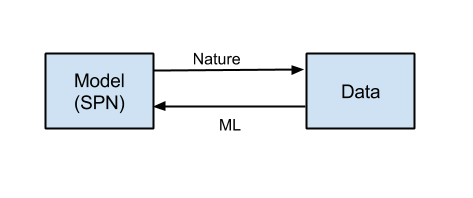
\includegraphics[width=0.5\textwidth]{ml}
\caption[ML inverse problem formulation]{ML inverse problem formulation}
\label{fig:ml}
\end{figure}



\subsubsection{Point estimates}
The experimental data are more formally a matrix $D$ with an element $D_{ik}$ being
the number of tokens accumulated in the $k$-th FA in the $i$-th
sample. Since we have multiple
realisations of Bernoulli trials, the success probabilities can also be
thought of as success probabilities in binomial distributions. The
Maximum Likelihood point estimator for binomial success probabilities
is given for the $i$-th decision corresponding to the $i$-th FA,
\begin{equation*}
\hat{p_i} = \frac{k_i}{n_i}
\end{equation*}
where $k_i$ is the number of successes and $n_i$ is the number of
trials. If we extract information about the number of successes and
number of trials for each binary decision in the process from data
that are different realisation of the process, then we can
straightforwardly compute the success probabilities.

If we a take a specific sample (a row from data matrix $D$) then the
number of successes for an FA is simply the number of tokens of
this FA in the sample since those are the tokens that when faced with
the decision of whether to get stored as that FA or continue to form
longer FAs they chose the former. Success and failure are arbitrarily
assigned to staying and continuing respectively. The number of trials
is the number of all the tokens that reached that FA intermediary, both
the ones that stayed \textit{and} the ones that continued. Since this
is an iterative process the ones that continued are the number of
tokens that made it to the sinks after the FA(the ones on the right as
we look at the Petri Net model picture,
Figure~\ref{fig:fa_elongation_full}). To illustrate this consider a
sample which could be a row from our data matrix $D$: $\{C_{12}=5,
C_{14}=10, C_{16}=34, C_{18}=23, C_{20}=3, C_{22}=5\}$. The ML
estimator for the $i$-th FA product in that sample will be:
\begin{equation*}
\hat{p_i} = \frac{C_i}{\sum_{n \geq i} C_n}
\end{equation*}
The success probabilities $p_1$ to $p_6$ for the above sample, with $p_1$ corresponding to
the first binary decision and $C_{12}$, $p_s$ to the second decision
and $C_{14}$ and so on, are:
\begin{align*}
\hat{p_1} & = 5/(5+10+34+23+3+5) = 0.0625\\
\hat{p_2} & = 10 / (10+34+23+3+5) = 0.1333\\
\hat{p_3} & = 34 / (34+23+3+5) = 0.523\\
\hat{p_4} & = 23 / (23+3+5) = 0.742\\
\hat{p_5} & = 3 / (3+5) = 0.375\\
\hat{p_6} & = 1
\end{align*}
This is for one sample but if all the samples are from the same
population, we can combine the successes/trials data from all
samples and generalise the ML success probability estimation for the
$i$-th FA product as:
\begin{equation*}
\hat{p_i} = \frac{\sum_k D_{ki}}{\sum_k \sum_{n\geq i} D_{kn}}
\end{equation*}
We assume that the columns of data matrix D are ordered according to
the order of FAs in the system.

At the end, the relative proportions of the transitions are important not the timeframe of generating the iterations in our process. We can therefore
use the calculated success probabilities as the rates of the
transitions related to the binary decision(s). So for example if
$\hat{p_3}\approx0.82$ then the rates of the transitions corresponding to the
binary decision for the 3rd FA, $C_{16}$, will be: rate of transition
for $C_{16}$ storage (success) $0.82$ and rate of transition for
$C_{18}$ formation (failure) $0.18$($1-P(success)$).


\subsubsection{Profiles}
In the previous section we presented a method to get point estimates for the success
probabilities guiding the binary decisions taking place during the
elongation process. We did that by considering the success
probabilities that maximise the likelihood function $L(D|p_i)$ for
the $i$-th FA and data $D$ being the number of successes and number of
trials. In this section I will present a likelihood function for the
entire process which comes naturally by thinking of the process as
before as a sequence of series of Bernoulli trials. We then use this
likelihood function to present a method for calculating the profiles
of the parameters.

The data from one of the samples can be seen as one realisation of the
stochastic process with the numbers of tokens at each FA being the
outputs of the series of Bernoulli trials that make up one realisation
of the entire process. Each series of Bernoulli trials describes the
journey of one token through the net which ends when it finds a
sink. If for example the token ends up at the third sink that means
that the outcome of the series of Bernoulli trials was: fail, fail,
success. Therefore the data consisting of the number of tokens that
ended up at each FA gives us a history of the series of trials that
happened during that realisation of the process. Consider the
following sample $\{C_{12}=5, C_{14}=10, C_{16}=34, C_{18}=23,
C_{20}=3, C_{22}=5\}$ which is one realisation of the process from
the start until reaching a dead-state. The numbers tell us the 'fate'
of each of the tokens that went through the net during that
realisation of the process, 5 tokens made the decision to stay at the
first trial- [success]- , 10 tokens made a decision to continue on the
first decision and then to stay on the second decision- [fail,
sucess]-, 34 tokens continued on the first two decision and stayed on
the third- [fail, fail, success], and so on. We can therefore calculate
the probabilities for each FA product sinks as follows:
\begin{align}
P(C_{12}) &= p_1 \nonumber\\
P(C_{14}) &= (1-p_1)p_2 \nonumber\\
P(C_{16}) &= (1-p_1)(1-p_2)p_3 \nonumber \\
P(C_{18}) &= (1-p_1)(1-p_2)(1-p_3)p_4 \nonumber\\
P(C_{20}) &= (1-p_1)(1-p_2)(1-p_3)(1-p_4)p_5 \nonumber\\
P(C_{22}) &= (1-p_1)(1-p_2)(1-p_3)(1-p_4)(1-p_5)p_6 \nonumber\\
\label{eq:param_cor}
\end{align}
The entire process can then be seen as a multinomial draw with 6
outcomes,  $\{C_{12}, C_{14}, C_{16}, C_{18}, C_{20}, C_{22}\}$, with
their respective probabilities given above and with the number of
trials being the number of tokens that ended up in sinks for that
particular realisation of the process. This gives the likelihood
function of the data given the success probabilities as
probability mass function of the multinomial distribution:
\begin{equation*}
L(D|\mathbf{\theta}) = f(C_{12},\dots, C_{22}; n ; P(C_{12}), \dots,
P(C_{22})\}) =
\end{equation*}

Using the likelihood function for the entire process we can find the
posterior of the initial success probabilities $p_1$ to $p_6$,
\begin{equation*}
P(\{p_i\} | D) \sim L(D | \{p_i\}) P(\{p_i\})
\end{equation*}
where the data $D$ is simply the outputs of one realisation of the
process or the counts at each sink and $P(\{p_i\})$ are the priors of
the parameters. If we assume uniformative priors the above parameter
posterior simply becomes: $P(\{p_i\} | D) \sim L(D | \{p_i\})$. Since
the parameters are not exactly the parameters of the multinomial but
they are only related through Equations~\ref{eq:param_cor} an analytic
solutions is not very attractive but since it is still a small problem
we can resort to a simple simulation scheme to sample from the required
posterior. I used the standard Metropolis-Hastings Markov Chain Monte Carlo method to
sample from the posterior as given above starting from a random point
in parameter space and a symmetric normal proposal distribution with
mean the previous accepted guess and an arbitrary chosen variance.


\subsection{Results}
\label{sec:results}
In this section we use the methods described previously to analyse and
calculate the success probabilities from a real experimental
dataset. The dataset comes from an experimental study for the effects
of a treatment on the profiles of Fatty Acids on mice. FAs
were extracted from brown adipose tissue from 91 mice subjected to 5
levels of treatment. The FAs in the samples include both the free FAs
and FAs that were cleaved from more complex lipid products. The amount
of the extracted lipid species was measured with Gas Chromatography
and a Flame ionization detector that gave relative intensities of each
product. Each sample contained measurements from 34 FAs products that
were identifiable in the measurements. From those 34 only 6 correspond
to the outputs of our process of interest, namely the even-chain saturated FAs
C12:0, C14:0, C16:0, C18:0, C20:0, C22:0. This guided the model
construction choices with sink outputs appearing at FAs with only these
lengths and the entire process stopping at C22. The outputs of the net model are integer number of tokens accumulated
at each of the sinks while the experimental
data are relative intensities which are continuous numbers. In order
to be able to compare with the data for the tuning of the parameters the
experimental data were transformed from relative intensities to
relative absolute numbers. A sample of relative
intensities $\mathbf{s} = \{s_1, s_2, s_3, s_4, s_5, s_6\}$ became a
transformed sample $\mathbf{ts} = \{ ts_i | ts_i = \lfloor s_i /
min(\mathbf{s}) \rfloor \}$.
 Since we are only interested in the
relative proportions of the outputs going from relative intensities to
relative numbers should not affect the outcome.

Point estimates of the  success probabilities calculated with from the
Control(treatment level 0)
subset of the real dataset can be seen in
Table~\ref{tab:param_estimates}. We then applied Baysian Hierarchical
Clustering (BHC) to the samples in the dataset to investigate changes
in the parameters in the different groups. The clustering algorithm
gave back 4 clusters. The centroid of each of the 4 clusters was used
to calculate point estimates of the parameters. The centroids for each
cluster can be seen in Figure~\ref{fig:clusters} and the calculated
success probabilities for each cluster can be seen in
Table~\ref{tab:param_estimates_clusters}.

\begin{table}
\centering
    \begin{tabular}{ccc}
    Parameter & Value \\ \hline
    $p_1$ &  0.0003000656 \\
    $p_2$ & 0.0400323889\\
    $p_3$ &  0.8235217126\\
    $p_4$ &  0.9888339514\\
    $p_5$ &  0.778597786 \\
    $p_6$ &  1.0
    \end{tabular}
\caption{Success probabilities estimated from the Control samples in
  the dataset.}
\label{tab:param_estimates}
\end{table}

\begin{figure}[htbp!]
\centering
\includegraphics[width=1.1\textwidth]{clusters}
\caption[ML inverse problem formulation]{Centroids for each of the
  four cluster discovered in the data with BHC.}
\label{fig:clusters}
\end{figure}

\begin{table}
\centering
    \begin{tabular}{ccccccc}
Parameter&  Cluster 1& Cluster 2& Cluster 3& Cluster 4 \\ \hline
$p_1$ & 0.0008979348 & 0.0013392857 & 0.0011865915& 0.0008532423 \\
$p_2$ & 0.04284002 & 0.04380867 & 0.05435105 & 0.04312553 \\
$p_3$ & 0.7984351 & 0.8092567 & 0.8483040 & 0.8420348 \\
$p_4$ &  0.9906832 & 0.9901961 & 0.9896480 & 0.9887006 \\
$p_5$ & 0.8333333 & 0.7500000 & 0.8000000 & 0.7500000 \\
\end{tabular}
\caption{Point estimates for the success probabilities for each cluster.}
\label{tab:param_estimates_clusters}
\end{table}




\subsection{Stochastic $\pi$-calculus implementation}
In this section I present a stochastic pi-calculus version of the
model which is specifically written in its SPiM variant which extends
the traditional pi-calculus first by introducing explicitly time which
is needed for quantitive analysis of biochemical networks and also by
adding operational semantics in terms of an Abstract Machine and a
graphical representation language. The SPiM code is given for the
processes making up the system to introduce further some of the
concepts of the SPiM language.

The SPiM graphical representation of the model can be seen in
Figure~\ref{fig:spim_graph}. Each component of that graph is a
stochastic pi-calculus process and edges between them indicate that
one one of them can evolve into the other. The nature of the model is
different from the equivalent model given in the previous section. The
evolution of every species represented by a stochastic pi-calculus
process is defined independently. We start the computation by running 100
\texttt{Acyl\_CoA} processes and 30 \texttt{Malonyl\_CoA} processes:

\begin{verbatim}
run(100 of Malonyl_CoA() | 30 of Acyl_CoA())
\end{verbatim}

The initial reaction of the system creating the $C_4$ product is represented as
communication by channel \texttt{form6} between \texttt{Acyl\_CoA} and
\texttt{Malonyl\_CoA} processes. Once the communication happens the
\texttt{Acyl\_CoA} process evolves into the  \texttt{Acyl\_CoA\_4}
process while \texttt{Malonyl\_CoA} process goes to the empty
process(gets consumed). After that all the processes corresponding
FAs between $C_6$ and $C_{10}$ only have one communication option,
communicate via the appropriate channel with a \texttt{Malonyl\_CoA}
process and then evolve into a process corresponding to a longer
FA. For example process \texttt{Acyl\_CoA\_8}:

\begin{verbatim}
and Acyl_CoA_8() = ?form10; Acyl_CoA_10()
\end{verbatim}

After that all the processes corresponding to intermediaries for longer
than $C_{10}$ FAs have two communication options corresponding to the familiar
stay-continue stochastic decision that we have seen in the previous section, they
can either communicate with a \texttt{Malonyl\_CoA} process and evolve
into a process corresponding to a longer FA while the
\texttt{Malonyl\_CoA} process terminates or do a delay and evolve into
their corresponding FA product. The FA products which are modelled as
empty processes could have been ignored since they do not interact
further with any other processes but they were kept there
intentionally to keep track of their numbers.

\begin{figure}[htbp!]
\centering
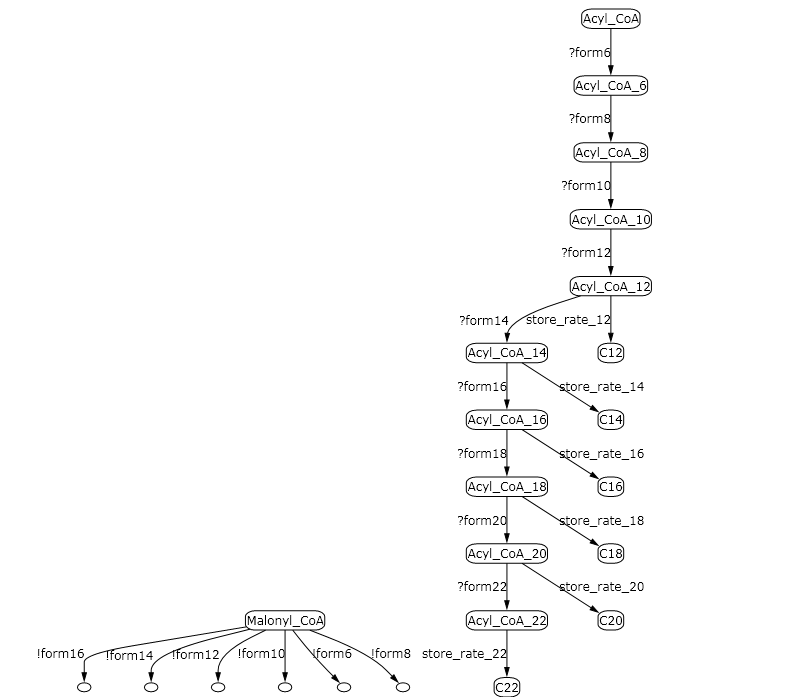
\includegraphics[width=1.0\textwidth]{spim_graph}
\caption[SPiM graph]{SPiM graph}
\label{fig:spim_graph}
\end{figure}

\begin{verbatim}
let Malonyl_CoA() =
(
	do !form6; ()
	or !form8; ()
	or !form10; ()
	or !form12; ()
	or !form14; ()
	or !form16; ()
)
and Acyl_CoA() = ?form6; Acyl_CoA_6()
and Acyl_CoA_6() = ?form8; Acyl_CoA_8()
and Acyl_CoA_8() = ?form10; Acyl_CoA_10()
and Acyl_CoA_10() = ?form12; Acyl_CoA_12()
and Acyl_CoA_12() =
(
	do ?form14; Acyl_CoA_14()
	or delay@store_rate_12; C12()
)
and Acyl_CoA_14() =
(
	do ?form16; Acyl_CoA_16()
	or delay@store_rate_14; C14()
)
and Acyl_CoA_16() =
(
	do ?form18; Acyl_CoA_18()
	or delay@store_rate_16; C16()
)
and Acyl_CoA_18() =
(
	do ?form20; Acyl_CoA_20()
	or delay@store_rate_18; C18()
)
and Acyl_CoA_20() =
(
	do ?form22; Acyl_CoA_22()
	or delay@store_rate_20; C20()
)
and Acyl_CoA_22() = delay@store_rate_22; C22()
and C12() = ()
and C14() = ()
and C16() = ()
and C18() = ()
and C20() = ()
and C22() = ()

run(100 of Malonyl_CoA() | 30 of Acyl_CoA())
\end{verbatim}


\section{Extended model of FA synthesis}
In the previous section I presented Petri Net and stochastic
pi-calculus implementations of a
simplified view of FA elongation/synthesis. In this section I
will present a Petri net implementation of an extended model which
captures one of the main control regulatory mechanisms between FA
biosynthesis and other general metabolic
machinery of the cell. The first and commited step in the FA
biosynthesis pathway is the conversion of acetyl-CoA to Malonyl-CoA
through the action of acetyl-CoA carboxylase. Acetyl-CoA carboxylase
is inactivated by AMPK protein kinase in mammals. In the well-fed
state AMPK is itself inactivated which leads to an increase in the
flow of Acetyl-CoA to Malonyl-CoA and since this is an irreversible
reaction to the FA biosynthesis pathway.
Also in conditions of high glucose
concentration isocitrate dehydrogenase is inhibited so Acetyl-CoA only
does the first step of the Krebs cycle when Citrate is produced. Since
Citrate cannot go any further in the cycle it starts to accumulate
until it starts to diffuse from the mitochondrion into the cytosol
where it becomes Acetyl-CoA again and acts as precursor for FA
biosynthesis. The net effect of these two factors is that more Acetyl-CoA will
flow towards the FA biosynthesis than go towards the
Kreb cycle and the Respiratory chain to produce energy because the
immediate energy requirements are low (high ATP).

\citet{nielsen2009systems} experimentally confirmed that
this regulatory mechanism is conserved in yeast through the action of
Snf1 which the yeast analog of the mammalian AMPK and they also
produced Flux Balance models to capture the
change in flows in the system throught the action of protein kinase
Snf1. Here we provide a Petri Net implementation of the above
regulatory scheme as an extension to the basic model we presented
in the previous section.

\subsection{Petri Net implementation}
The Petri Net implementation of the above mentioned regulatory
mechanism as an extension to the basic model presented before can be
seen in Figure~\ref{fig:pn_ext}. The net starts with an empty
transition feeding into glucose which can be thought of as an
interface to the environment. That could for example be used to model
glucose intake from the diet. Then after that the action of every pathway
is condensed into a single transition except FA
biosynthesis/elongation for which we use the basic model developed
previously. After the initial glucose intake transition, glucolysis is
represented by a transition from Glucose to Pyruvate and then
Acetyl-CoA which plays the central role in this regulatory
mechanism. Acetyl-CoA has a decision of whether to flow towards FA
biosynthesis represented by transitions to place \texttt{FAsyn}
or flow towards the TCA cycle and further energy production which is
represented by a transition to the \texttt{TCA}
place (red box in Figure~\ref{fig:pn_ext}). The \texttt{TCA}  place represents the combined
effect of the TCA cycle and the respiratory chain which has as an
ouput 30 molecules of ATP. ATP can then be consumed by taking part in
a transition without any post-places. ATP consumption could for
example be used to model various energy requirements. FA biosynthesis/elongation
process is represented as before. The only difference
is that it now only has a single input which then leads to the two
inputs used in the basic version of the model (green box in Figure~\ref{fig:pn_ext}).
The main regulatory mechanism comes by making ATP a pre-place for the
Acetyl-CoA transition to \texttt{FAsyn} so that ATP levels can
influence the rate of that transition and hence the flow towards FA
biosynthesis.

\begin{figure}[htbp!]
\centering
\includegraphics[width=1.2\textwidth]{pn_ext}
\caption[Extended Petri Net model]{An extended version of the model}
\label{fig:pn_ext}
\end{figure}


\subsection{Model Parameters}
In this section I present a way to construct the
rate functions for the transitions out of Acetyl-CoA in order to get
the required regulatory behaviour based on ATP levels and a way to
find the rate parameters for the transitions from the \texttt{FAsyn} place
to the two main input points for the FA synthesis/elongation process.

Since we have not modelled enzymatic
activity explicitly but only through the transition rates, the effect that ATP has on the enzyme responsible
for the flow of Acetyl-CoA to FA synthesis will have to become an effect
on the rate of the corresponding transition. In order to introduce
that effect the rate function for the transition taking Acetyl-CoA to FA biosynthesis
becomes an increasing function of ATP. That by itself
is not enough since at high ATP levels the reaction rate not only
needs to be high but crucially higher than the TCA transition rate in order to
make the flow towards FA biosynthesis more favorable when Acetyl-CoA
is faced with the TCA/FA biosynthsesis decision. So, again, the
important fact here, since we do not consider the timeframe of the
process, is the ratio between these parameters. In order to achieve
that we can set up a basal rate for the two alternatives for a
base level of ATP for which they are both equally likely to
happen. Any deviations from that balanced level and the flow towards
FA biosynthesis becomes more or less likely. Let us consider a
constant base level of $ATPb$ ATP molecules and a variable $ATP$ for the number
of ATP molecules at any given time during the execution of the
model. An example of rate functions that meet our requirements are:
$\lambda_{TCA} = ATPb^{k}$ and $\lambda_{FAsyn} =
ATP^{k}$. When $ATP=ATPb$ the transition rates are equal so the
Acetyl-CoA flows with equal likelihood to TCA and FA
biosynthesis. The strength of the response to deviations is then:
\begin{equation*}
\left ( \frac{ATP}{ATPb}\right)^{k}
\end{equation*}
We can therefore control the strength of the response by tuning the $k$
parameter. For linear responses for example we can set $k=1$ which
will mean that a 2-fold increase in the ATP level from its base rate
results in a doubling of the
rate of the transition towards FA biosynthesis while the rate towards
TCA remains constant.

For the transition rates from \texttt{FAsyn} we can make a simple
stoichiometric argument to find the correct ratio between them that
will guide the flow towards those two input points of the FA
synthesis/elongation process. For every $C_2$ concatenation step we
need one Malonyl-CoA so for example if the process does 7 steps to
reach the $C_{16}$ then we would need 7 Malonyl-CoAs and 1
Acetyl-CoA. Since it is a stochastic process however we do not know in
advance how many steps each token will take through the net. We can
however find the expectation of the number of steps:
\begin{equation*}
E(steps)=\sum_{4 \leq i \leq 9} i \times P(i)
\end{equation*}
So on average we need $E(steps)$ Malonyl-CoAs for every one
Acetyl-ACP. We can set the transition rates towards these two starting
points to reflect that:
\begin{align*}
\frac{\lambda_{Malonyl\_CoA}}{\lambda_{Acetyl\_CoA}} = E(steps)
\end{align*}


